\section{Terminology and Definitions}

A well-defined learning problem involves a number of design choices, including selecting the type of training experience, the target function to be learned, a representation for this target function, and an algorithm to learn from the source of training experience [2]. In modelling a political participation process, a computer program is designed to approximate the likelihood of a person going to vote on election day. Ideally, for every instance with unknown political interest and willingness to participate, there is enough data of people of similiar demographics, socioeconomics and psychological traits to generalize from. This chapter defines key terminology and destinctions when learning from biased data. Basic design issues and approaches to supervised learning are covered, while conceptual elements of interest are introduced with regards to overfitting. The role of noise in the bias-variance decomposition will be analyzed and further broken down. sources of error.

\subsection{Sampling Bias}

Sampling bias is often referred to as selection bias or sample selection bias. I will stick to the more descriptive term sampling bias. It underlines the fact that the bias arises in how the data was sampled. Also, the use of the term becomes less ambiguous, because there exists another notion of selection bias in the context of model selection. This type of bias is usually referred to as bad generalization, where the performance of the selected hypothesis is overly optimistic. [input: convenience sampling]

It is usually difficult to draw a simple random sample from the population, due to cost and practical considerations such as no comprehensive sampling frame available

Although one could employ a census to measure the entire population, it is more common to take a sample of the population. A properly designed probability sample (see probability sampling) can be used to make estimates for not only the sample itself, but also for the underlying population from which it was selected. A probability sample is one in which each element of the (underlying) population has a known and non-zero chance of being selected. That is, every person has a chance to be included in the study and have his or her characteristics, opinions, etc., become part of the data. It should be noted that everyone does not have to have an equal chance of being selected – just a known non-zero chance of being selected. 
Probability samples have several desirable characteristics. They enable us to put a margin of error or confidence interval on our estimates – essentially a measure of how accurate the estimate is compared to the same estimate calculated on the full population. Probability samples make it possible to not only compare the sample to the population, but also to compare a sample from one population to a sample from another population,

\subsection{Representative Sample}

Some examples include sex, age, education level, socioeconomic status or marital status. Information collections with biased tendencies can't generate a representative sample.

Variables considered in the study must accurately reflect the populations characteristics. 

Consider \textit{attribute: income} of a subset of GBS participants. Statistical significance tests, e.g. Kolmogorov-Smirnov, Chi-Squared

\begin{figure}[ht]
	\begin{center}
		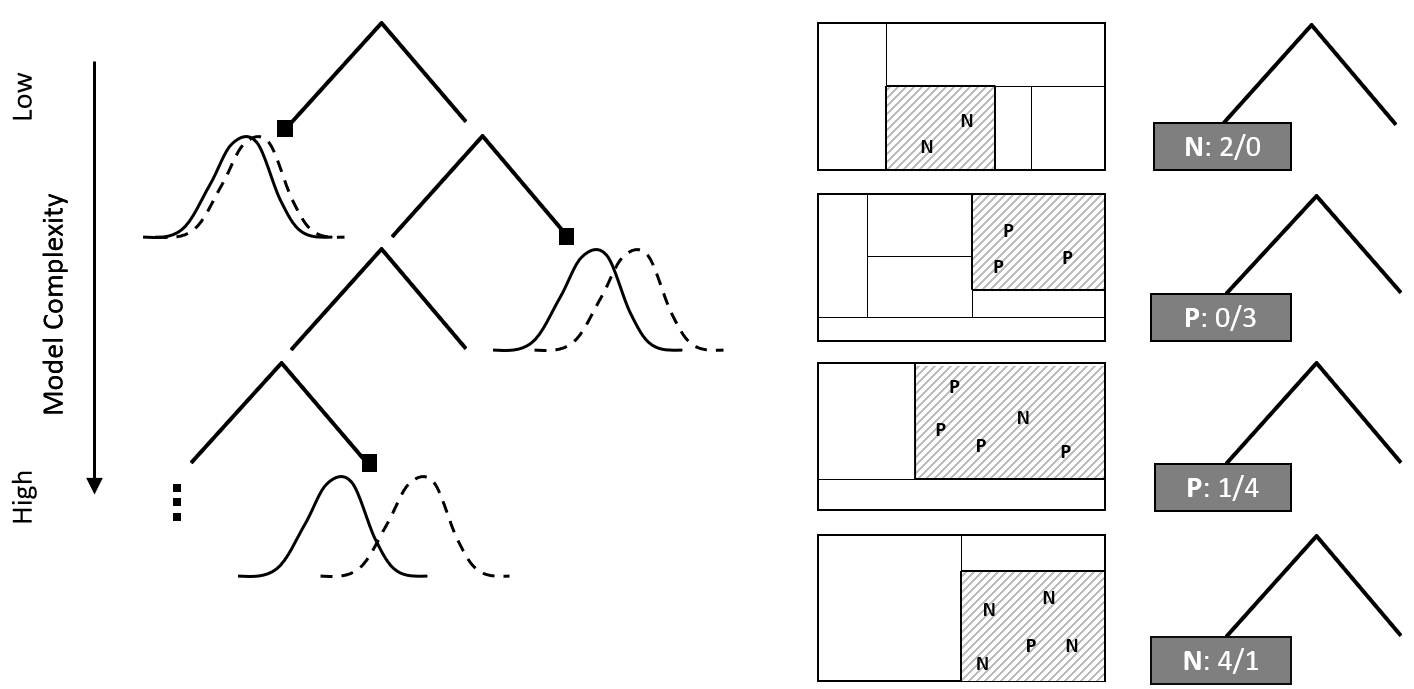
\includegraphics[scale=0.40,angle=0]{fig/tree3}
		\label{project}
		\caption{.}
	\end{center}
\end{figure}

Given a subset of GBS, similarity scores can be defined to evaluate the distance to reference distributions from GESIS. Kolmogorov-Smirnov tests or Chi-Squared assess the likelihood of an attribute of GBS  There are \(2^{|GBS|} = 2^{587}\) subsets of GBS. Evaluating every possible combination of GBS participants and its score is computationally intractable.

A well-defined learning problem where large polls (Umfragedaten) may contain valuable implicit regularities, requires a well-specified task, performance metric and source of training experience [2]. The MRS problem is now stated as a binary classification task with GESIS as positive class and GBS as negative class. Consider designing a computer program to learn to distinguish between . Using prior knowledge together with past experience to guide learning, a machine learning algorithm
is fed with data from games that have been played by chess grandmasters. From this information, the program will learn to apply certain functions to specific board states and make decisions about which move to play next.

Consider a randomly chosen survey participant, i.e. an instance of GBS or GESIS. If the poll indicates the or

Descriptive statistics can be used to 
 
No practical amount of data can distinguish between two distributions, thus instances of GBS can not be proven to come from GESIS. However, discriminative learning allows to infer the conditional probability of \textit{'instance of GBS/GESIS'} given the survey data within a probabilistic framework:


\subsection{The Problem of Overfitting}

By definition, statistical inference is taking the results of applying some sort of construct or model to specific data and then speculating that it would continue to perform well beyond the original observation range. Given a set of training samples \((x_i,y_i)\) find a single hypothesis \(h\) that "fits the data well": \(y_i = h(x_i)\) for most \(i\). The equation is characterized by a trade-off between goodness-of-fit and complexity of the hypothesis:

\begin{itemize}
\item if \(h\) is too simple, \(y_i = h(x_i)\) may not hold for many values of \(i\);
\item if \(h\) is too complex, it fits the data very well but will not generalize well on unseen data.
\end{itemize}


